\label{sec:model}

%\begin{figure}
%\centering
%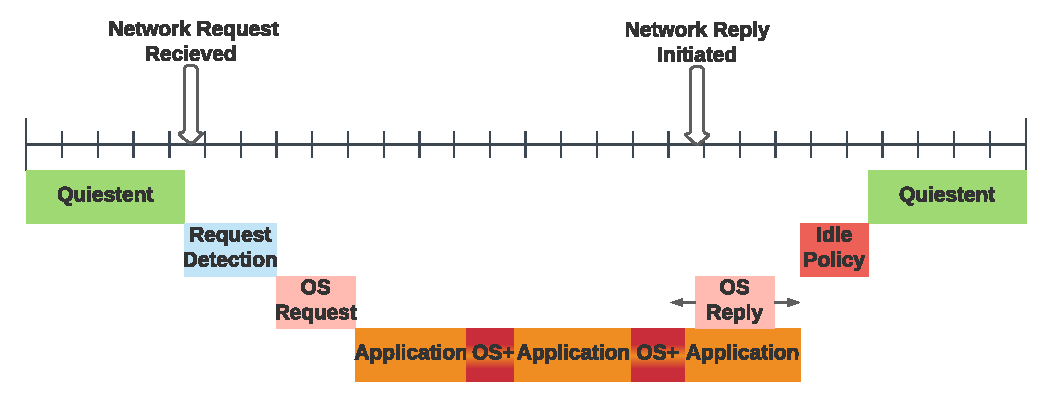
\includegraphics[width=0.5\textwidth]{figures/timeline_chart}
%\caption[]{Logical execution timeline for a single application request}
%\label{fig:timeline}
%\end{figure}

\subsection{Mathematical Framework}
%todo: some of this text should be in the intro as part of our contribution.
%An important goal for this work has been to create a useful framework for analyzing and exploring energy and performance impacts accounting for OS behavior.  The request timeline breakdown of Figure~\ref{fig:timeline} was our first step in choosing what to include and abstract from our knowledge of both OS software and the power management literature.  This was both to drive the quantitative study and enable the construction of a model that could be used by ourselves and others to explain and explore alternatives both software and hardware.   

In this section we briefly summarize our work in using our request time-line breakdown (Figure~\ref{fig:timeline} to develop a mathematical framework that can be used to explain and explore software and hardware effects.  In particular, we show how we model an open loop setting and explore the impacts of changes in the instruction path length and composition.  A more detailed discussion of the framework and how it can be used can be found in Appendix~\ref{sec:appendix}.   

Assuming a setting where the service time is less than or equal to the time between two requests, $\lambda$, we define:
%We begin by defining a breakdown of the service time between two consecutive requests arriving at an arrival rate (in queries/requests per unit time) $\lambda$ as:

$\boxed{\delta t = t_{\text{detect}} + t_{\text{osreq}} + t_{\text{app}} + t_{\text{idlepolicy}} + t_q} = \frac{1}{\lambda}$

where 

$\delta t$ = time between the arrivals of two consecutive requests and the remaining terms directly reflect the time-line components.  
%$t_{\text{detect}}$ = blah, $t_{\text{osreq}}$ = blah, $t_{\text{app}}$ = blah, $t_{\text{idlepolicy}}$ = blah, and $t_q$ = blah.

We group together the three terms that have a clear DVFS dependence as
$t_{\text{work}} \equiv t_{\text{osreq}} + t_{\text{app}} + t_{\text{idlepolicy}}$.  Excluding excluding detection and any quiescient time, and $t_{\text{latency}} \equiv t_{\text{detect}} + t_{\text{work}}$ for the total service time or latency for a request.

%Note that: $\delta t = \frac{1}{\lambda}$ or equivalently, $t_q = \left[\frac{1}{\lambda} - t_\text{work} - t_{\text{detect}}\right]^+$ where $[x]^+ = \max(x,0)$.


Similarly the total energy consumed during the inter-arrival time, $\delta t$ is:

$\boxed{E = P_\text{detect} t_{\text{detect}} + P_{\text{work}} \left[t_{\text{osreq}} + t_{\text{app}} + t_{\text{idlepolicy}}\right] + P_q t_q} = P_\text{detect} t_{\text{detect}} + P_{\text{work}} t_{\text{work}} + P_q t_q$

An important aspect of our model is our physically motivated abstraction of a processors DVFS setting, $\Delta$.  While a single value we reflect it having an independent impact on time (as a possible function of frequency) and power (as a possible function of voltage).  Specifically, we posit 
%power-law dependence of 
$t_{\text{work}}$ and $P_{\text{work}}$ as follows:

$t_{\text{work}} = A\frac{N_i}{\Delta^{1+\alpha}}$

$P_{\text{work}} = B \Delta^{2+\beta}$

where A, B are constants of proportionality, $N_i$ $=$ the total number of instructions and $\alpha$, $\beta$ are real-valued constants that describe the dependence on DVFS, $\Delta$.  This allows us, though $\alpha$ and $\beta$, to explore effects in which different instruction mixes, of the software, are affected in different ways with respect to time and energy by DVFS settings.  

%The core assumption here is that the various terms in figure \ref{timeline} don't overlap. We also assume that $\lambda$ is small enough that the service time is less than the inter-arrival time i.e. $t_{\text{service}} \leq \delta t$. This simple model also applies to the closed-loop case with the restriction that the arrival rate is now dependent on $t_{\text{service}}$. Lastly, this is a qualitative model that ignores stochastic effects (i.e. the full probability distribution of various terms). A quantitative extension of this analysis would cast this problem as a probabilistic graphical model and perform Bayesian inference for the underlying parameters.

Now to use the model we map
\begin{figure}
\centering
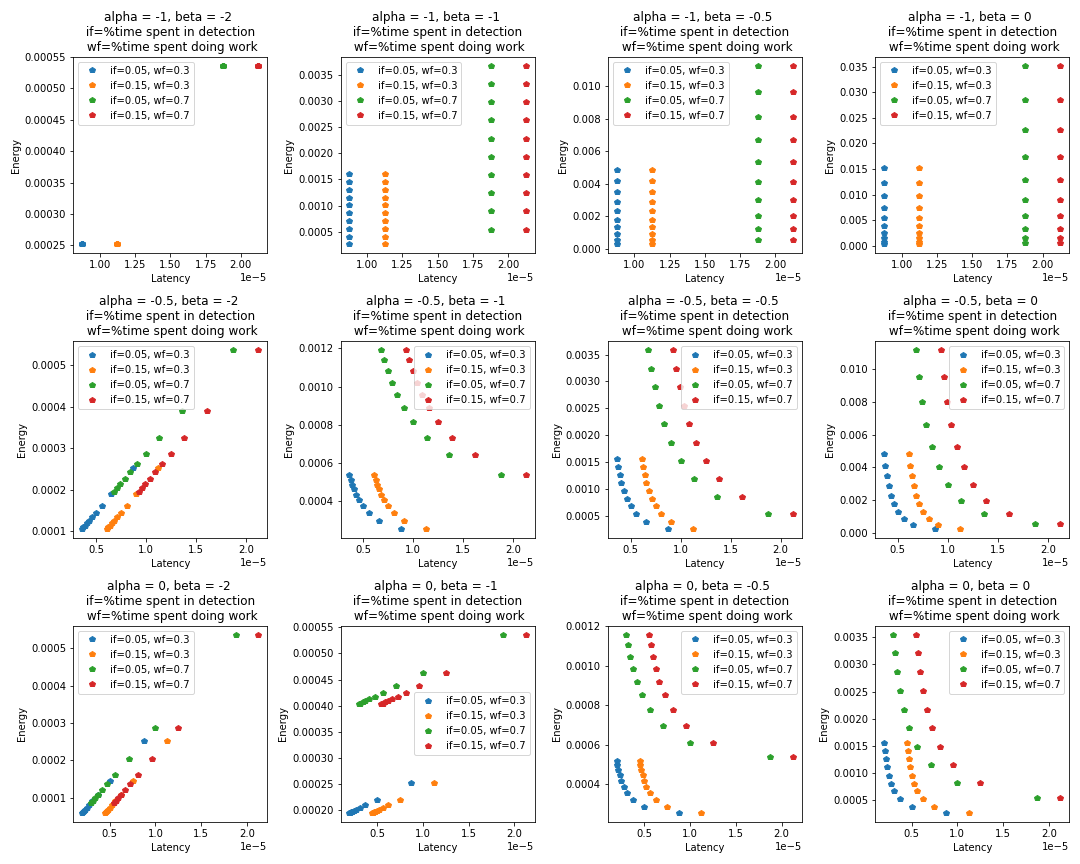
\includegraphics[width=.8\columnwidth]{figures/model_plots}
\caption[]{Simulated Plots}
\label{fig:simplots}
\vspace{-0.28in}
\end{figure}

